\section{Iluminación Global en Tiempo Real.}
\label{sec:interactive_gi_takes}
En esta sección se examinan algunos algoritmos para el cálculo de iluminación global en tiempos interactivos o \emph{real-time}. Iluminación indirecta con trazado de conos y vóxeles es revisada con detalle ya que esta técnica es de particular interés para este trabajo.

\subsection{Luces Puntuales Virtuales}
Una variedad de algoritmos para el cálculo de iluminación global se inspiran o hacen uso del concepto de \ac{VPL}. Este trabajo fue presentado por Keller en 1997 \cite{Keller:1997}.

\begin{figure}[H]
	\centering
	\begin{subfigure}[h]{0.35\textwidth}
		\centering
		\captionsetup{justification=centering}
		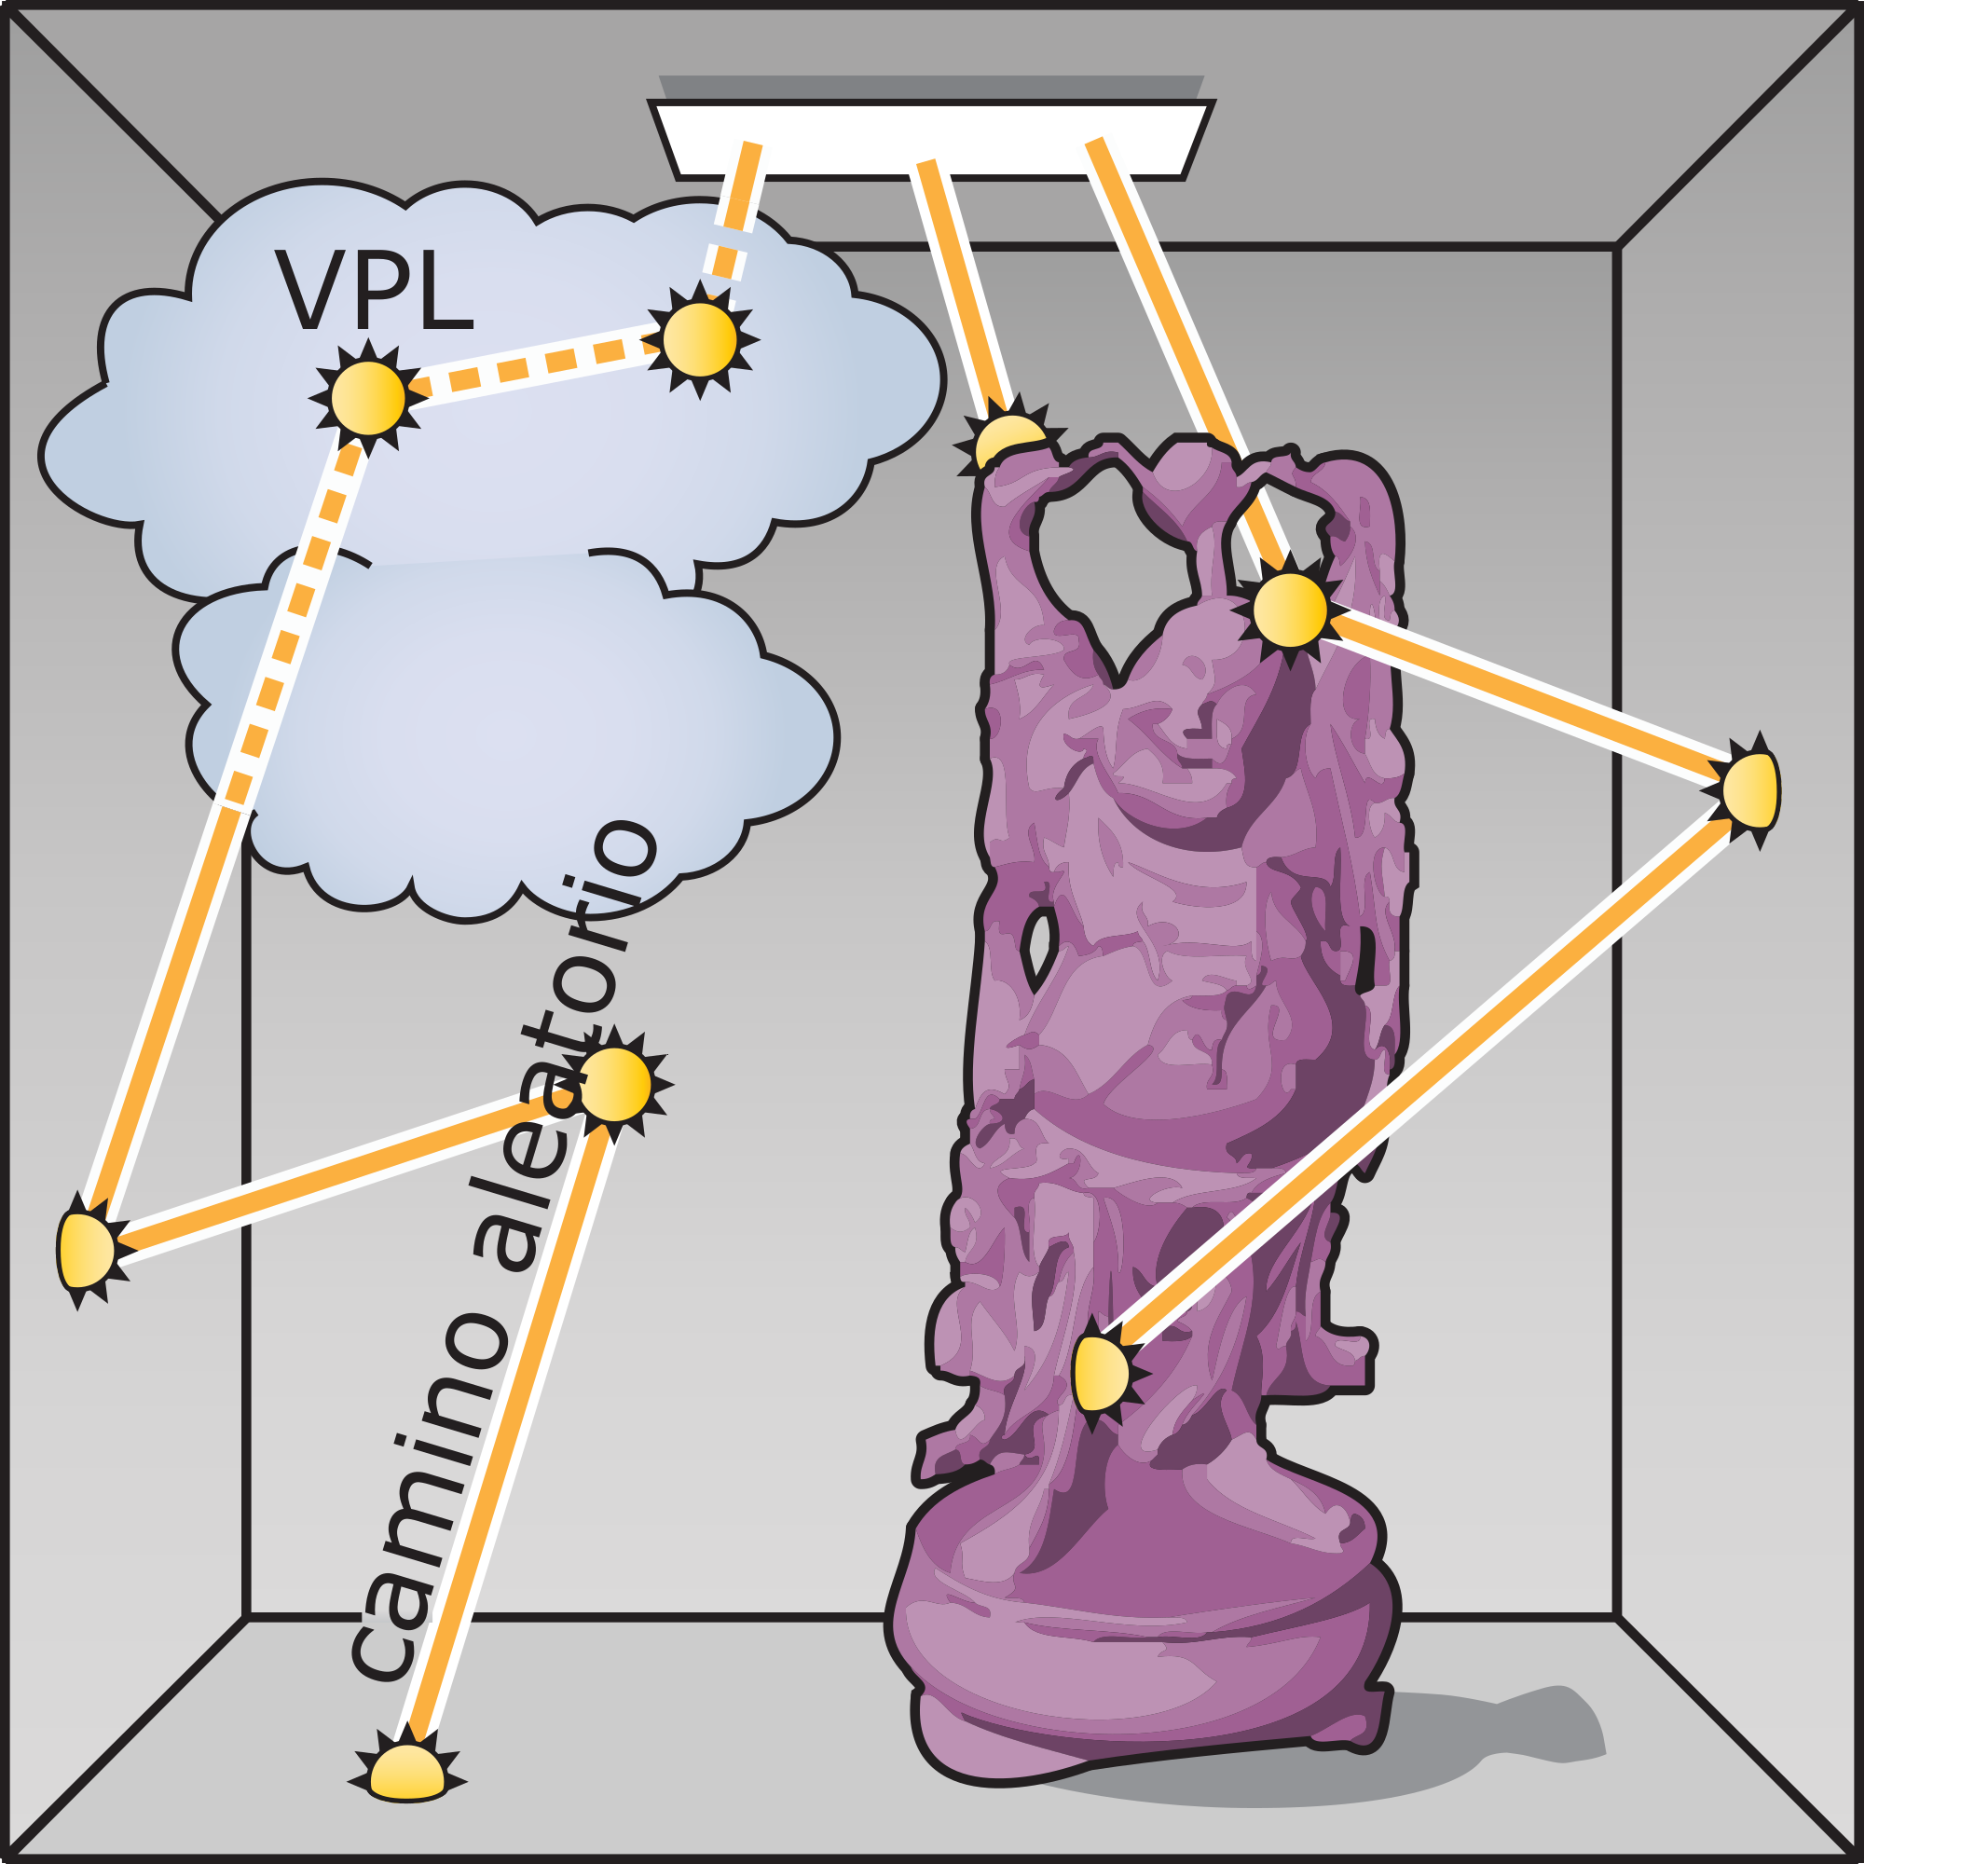
\includegraphics[width=\linewidth]{media/vpl1.png}
		\caption*{Generación de luces virtuales puntuales}
	\end{subfigure}
	\hspace{0.1\textwidth}
	\begin{subfigure}[h]{0.35\textwidth}
		\centering
		\captionsetup{justification=centering}
		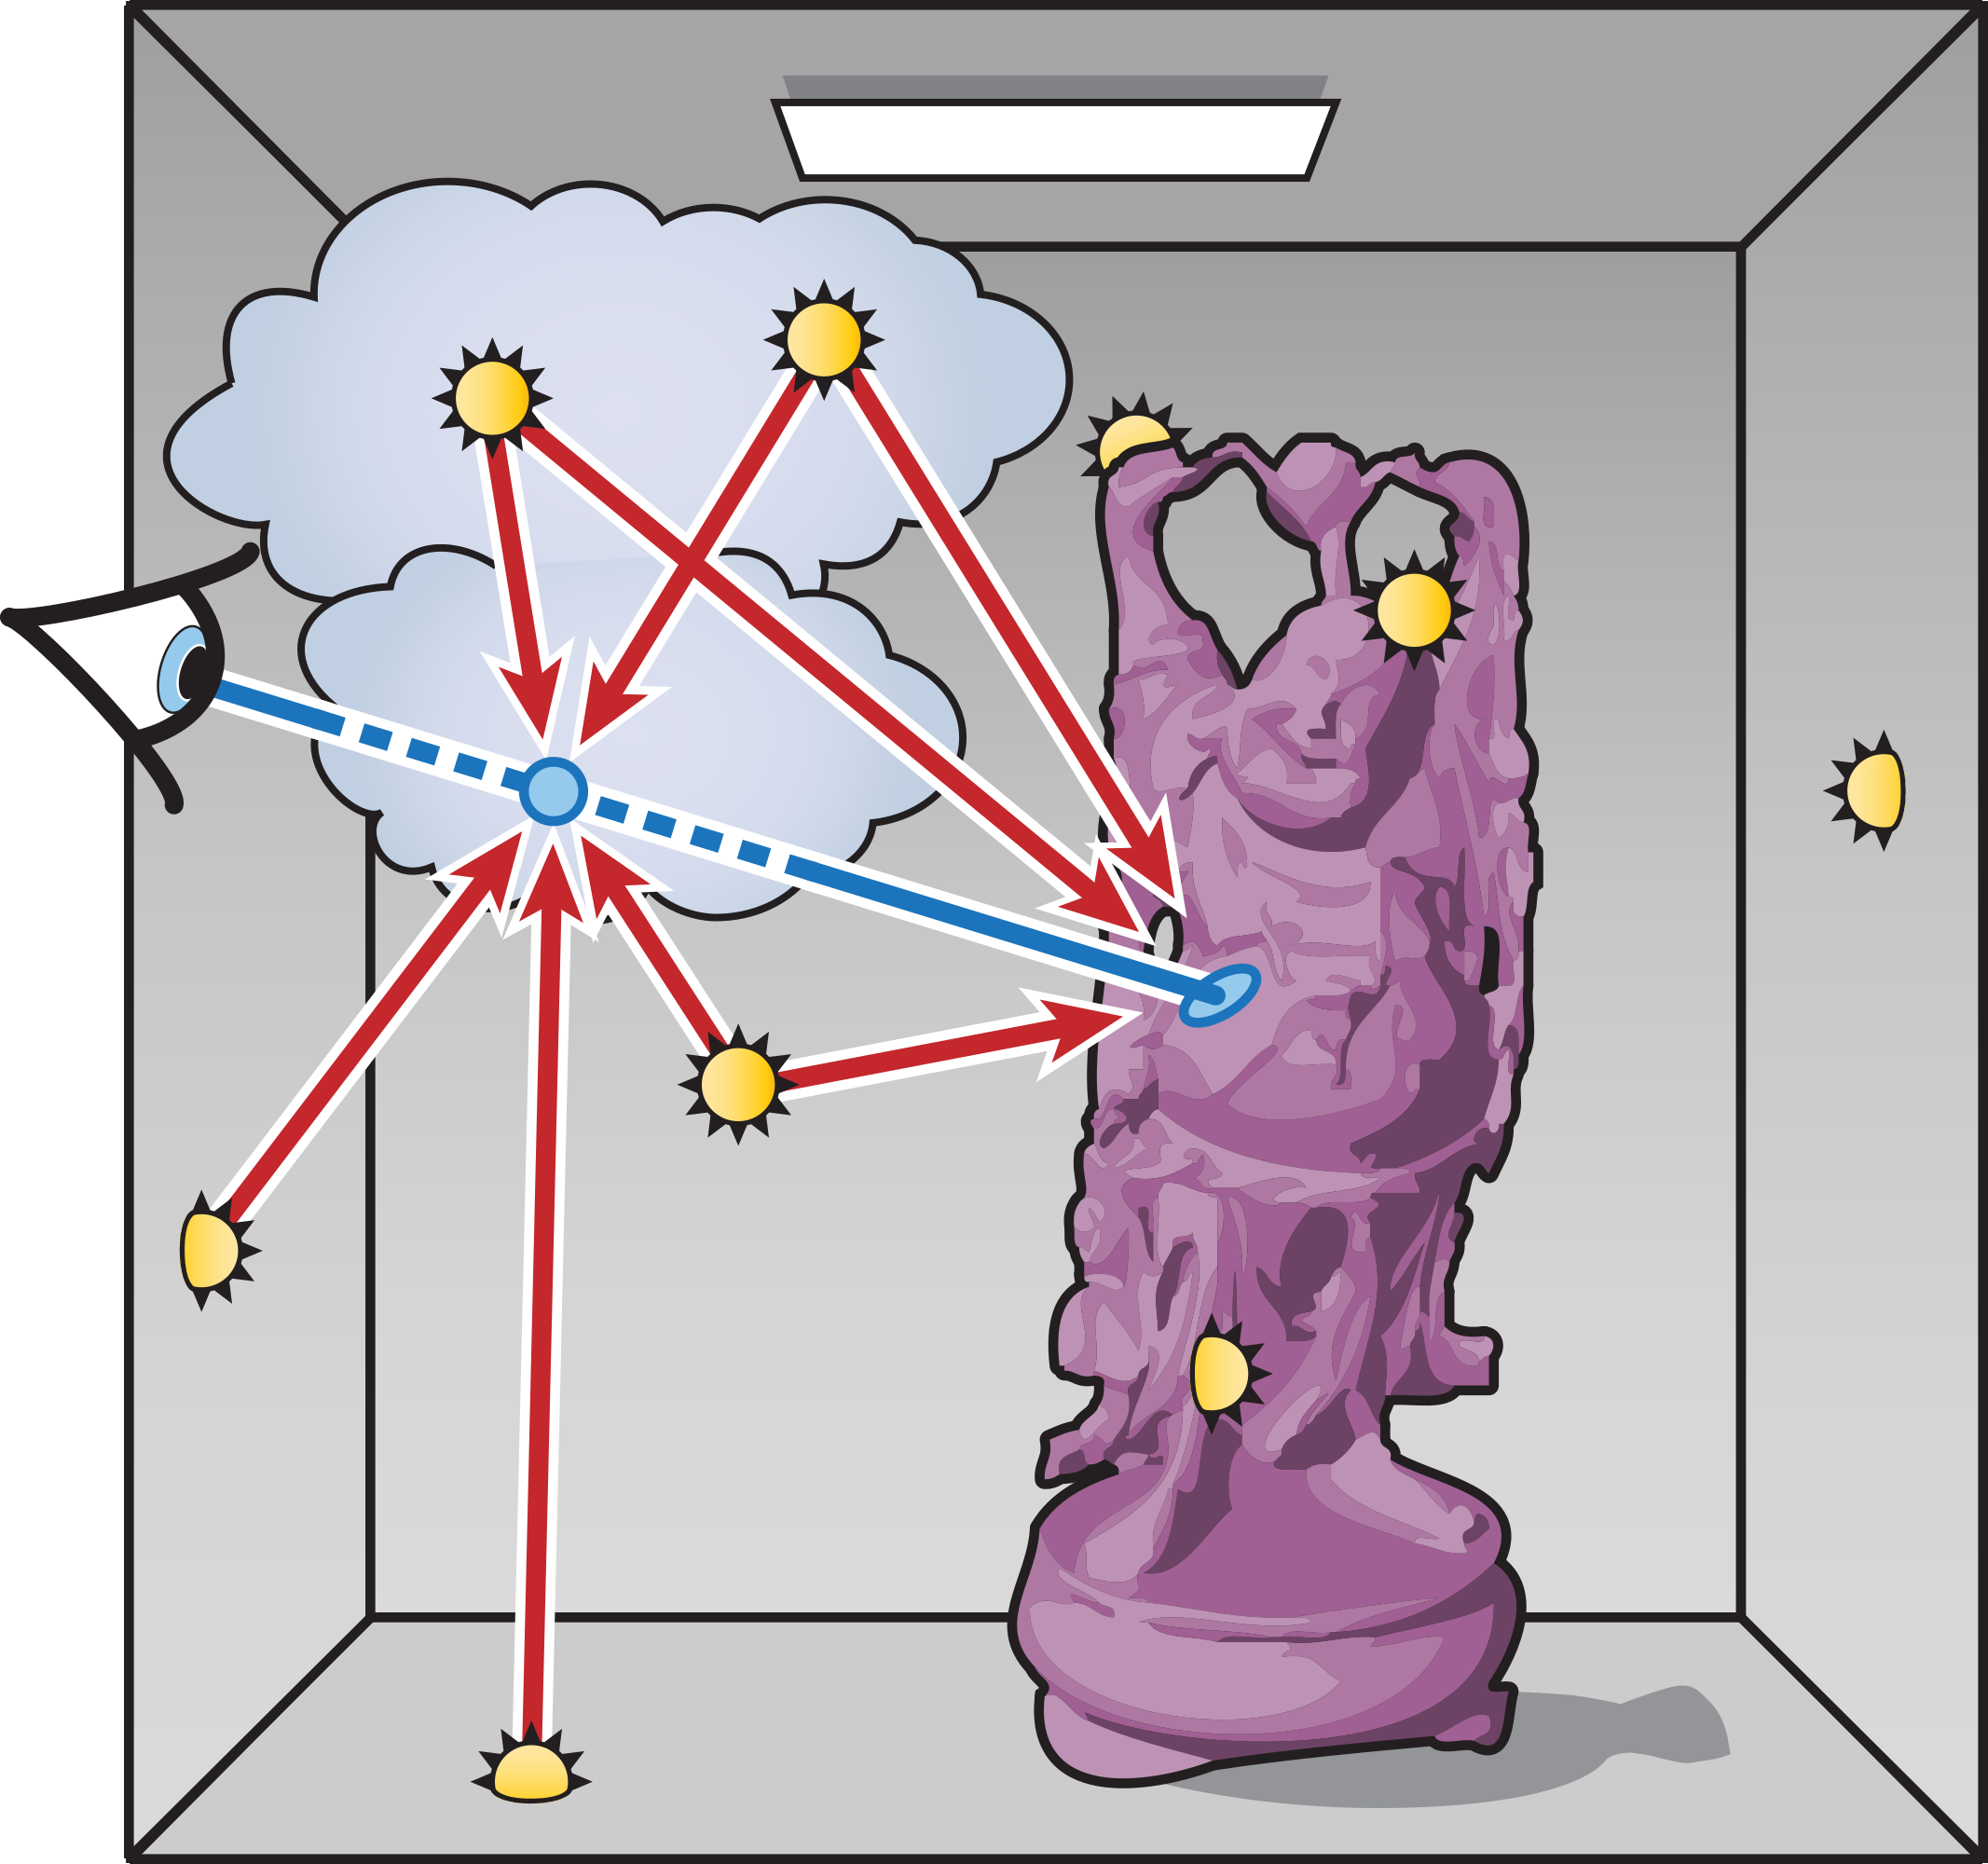
\includegraphics[width=\linewidth]{media/vpl2.png}
		\caption*{Aproximación de iluminación acumulada sobre un punto.}
	\end{subfigure}
	\caption{Pasos del algoritmo \ac{VPL} para la aproximación de iluminación indirecta \cite{Dachsbacher2014ManyLights}.}
	\label{fig:vpl_passes}
\end{figure}


En este algoritmo se aproxima la radiancia reflectada en escena utilizando un conjunto de luces virtuales. La radiancia que llega a un punto $x$ es aproximada por la radiancia que proviene de las luces virtuales. Pruebas de visibilidad para cada una de estas luces son realizadas utilizando técnicas de sombreado estándar y la radiancia proveniente de cada una de estas es almacenada en un buffer de acumulación. En la Figura \ref{fig:vpl_passes} se ilustra este algoritmo.
Las luces virtuales son generadas a partir de partículas lanzadas por las fuentes de luz principales utilizando la secuencia de Halton para el muestreo. En un principio, un número $n$ de partículas son generadas, como no toda la radiancia es absorbida algunas de estas partículas son reflejadas. Luego del primer rebote, uno número $p'n$ de partículas son reflejadas. Luego de $j-1$ reflexiones $p'^j$ son reflejadas. El número $p'$ es descrito por la siguiente ecuación:
\begin{equation}
    p' = \frac{\sum_{k=1}^{K} p_{d,k}|A_{k}|}{\sum_{k=1}^{K}|A_{k}|}
    \label{eq:reflected_vpls}
\end{equation} donde la escena es compuesta por $K$ elementos de superficie $A_{k}$ con una reflectividad promedio de $p_{d,k}$.

\subsection{Mapas de Sombras Reflexivo}
Otra técnica utilizada en varios algoritmos de iluminación global es \ac{RSM} o \emph{reflective shadow maps}. La técnica de \ac{RSM} fue presentada por Dachsbacher y otros en 2005 \cite{Dachsbacher:2005}.  Esta técnica está inspirada en mapeado de sombras como ya fue explicado anteriormente en \ref{subsec:shadowmapping}, se utiliza proyección desde la fuente de luz para determinar el primer rebote de luz. Al renderizar la escena desde el punto de vista de la fuente de luz, se entiende que todos los fragmentos en el mapa de sombras son los únicos fragmentos involucrados en el primer rebote de luz. En \ac{RSM} cada uno de los píxeles en el mapa de sombras es considerado una fuente de luz. Por cada píxel $p$ además de la profundidad $d_{p}$, se necesita almacenar posición $x_{p}$, normal $n_{p}$, y el flujo de radiancia reflectada $\Theta_{p}$. En la Figura \ref{fig:rsm_fbo} se puede observar el contenido de un \ac{RSM}.

\begin{figure}[H]
	\centering
	\begin{subfigure}[t]{.24\linewidth}
		\centering
		\captionsetup{justification=centering}
		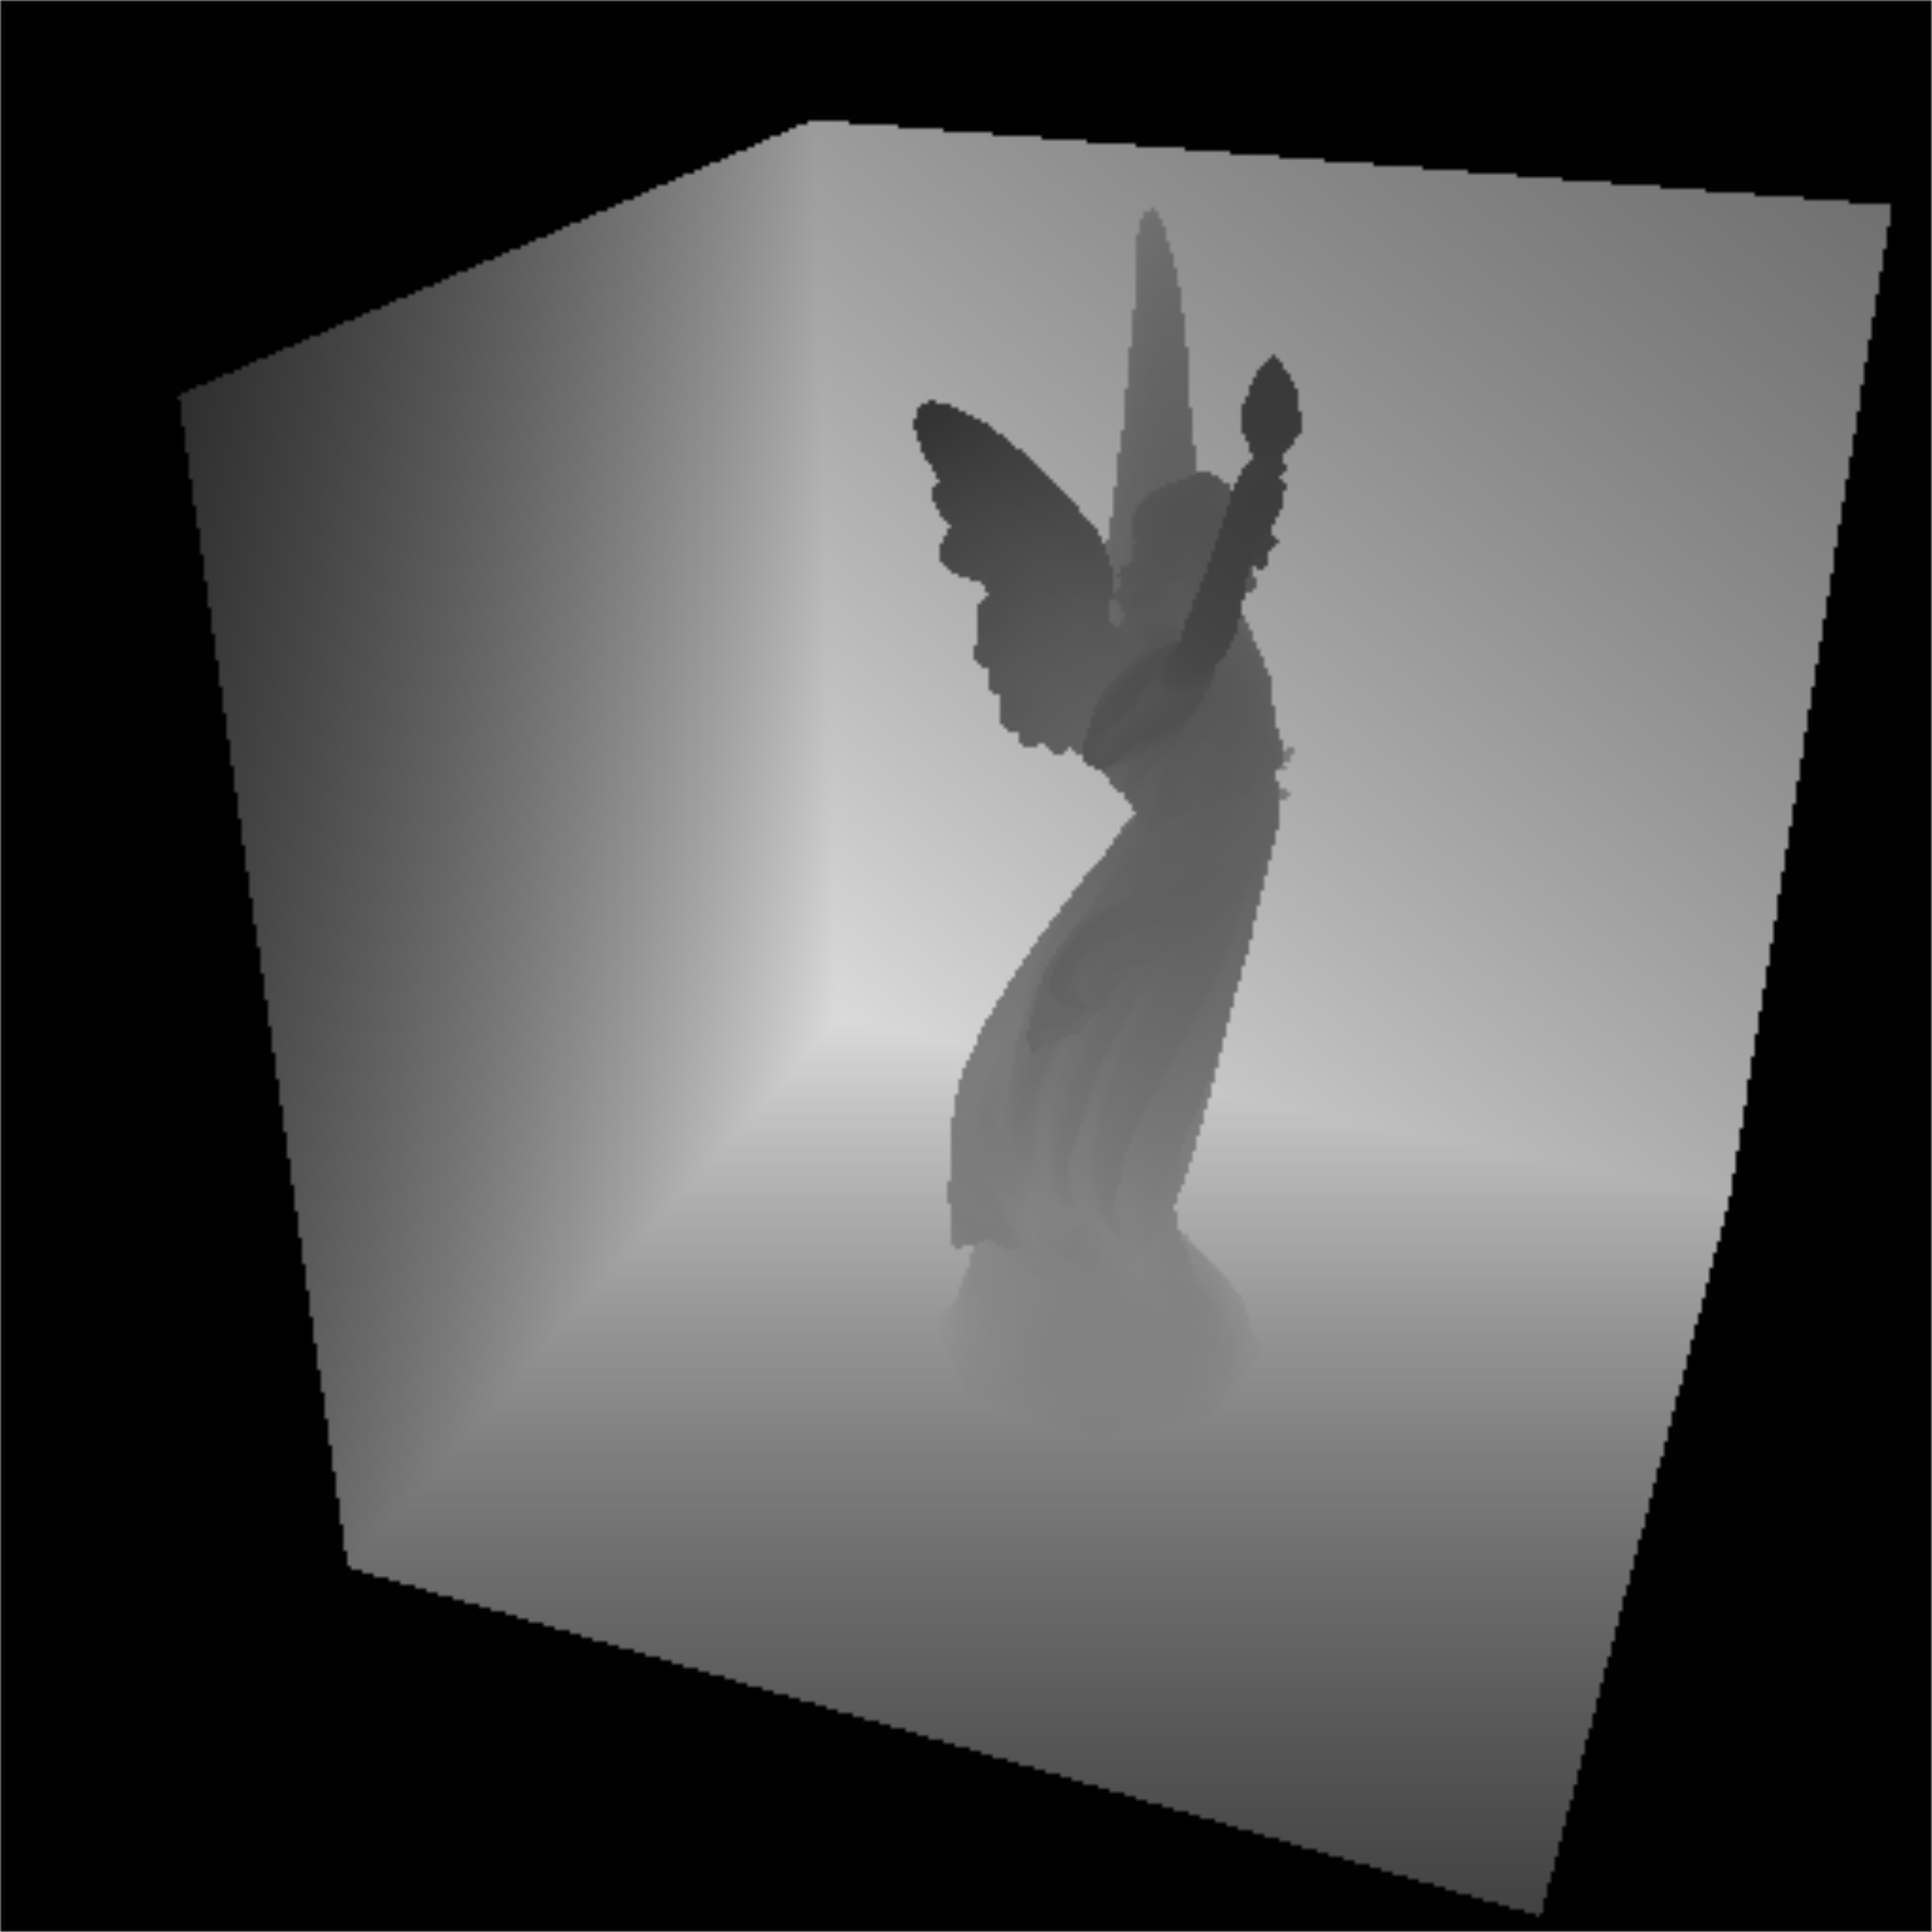
\includegraphics[width=\linewidth]{media/rsmd.png}
		\caption*{Profundidad.}
	\end{subfigure}
	\begin{subfigure}[t]{.24\linewidth}
		\centering
		\captionsetup{justification=centering}
		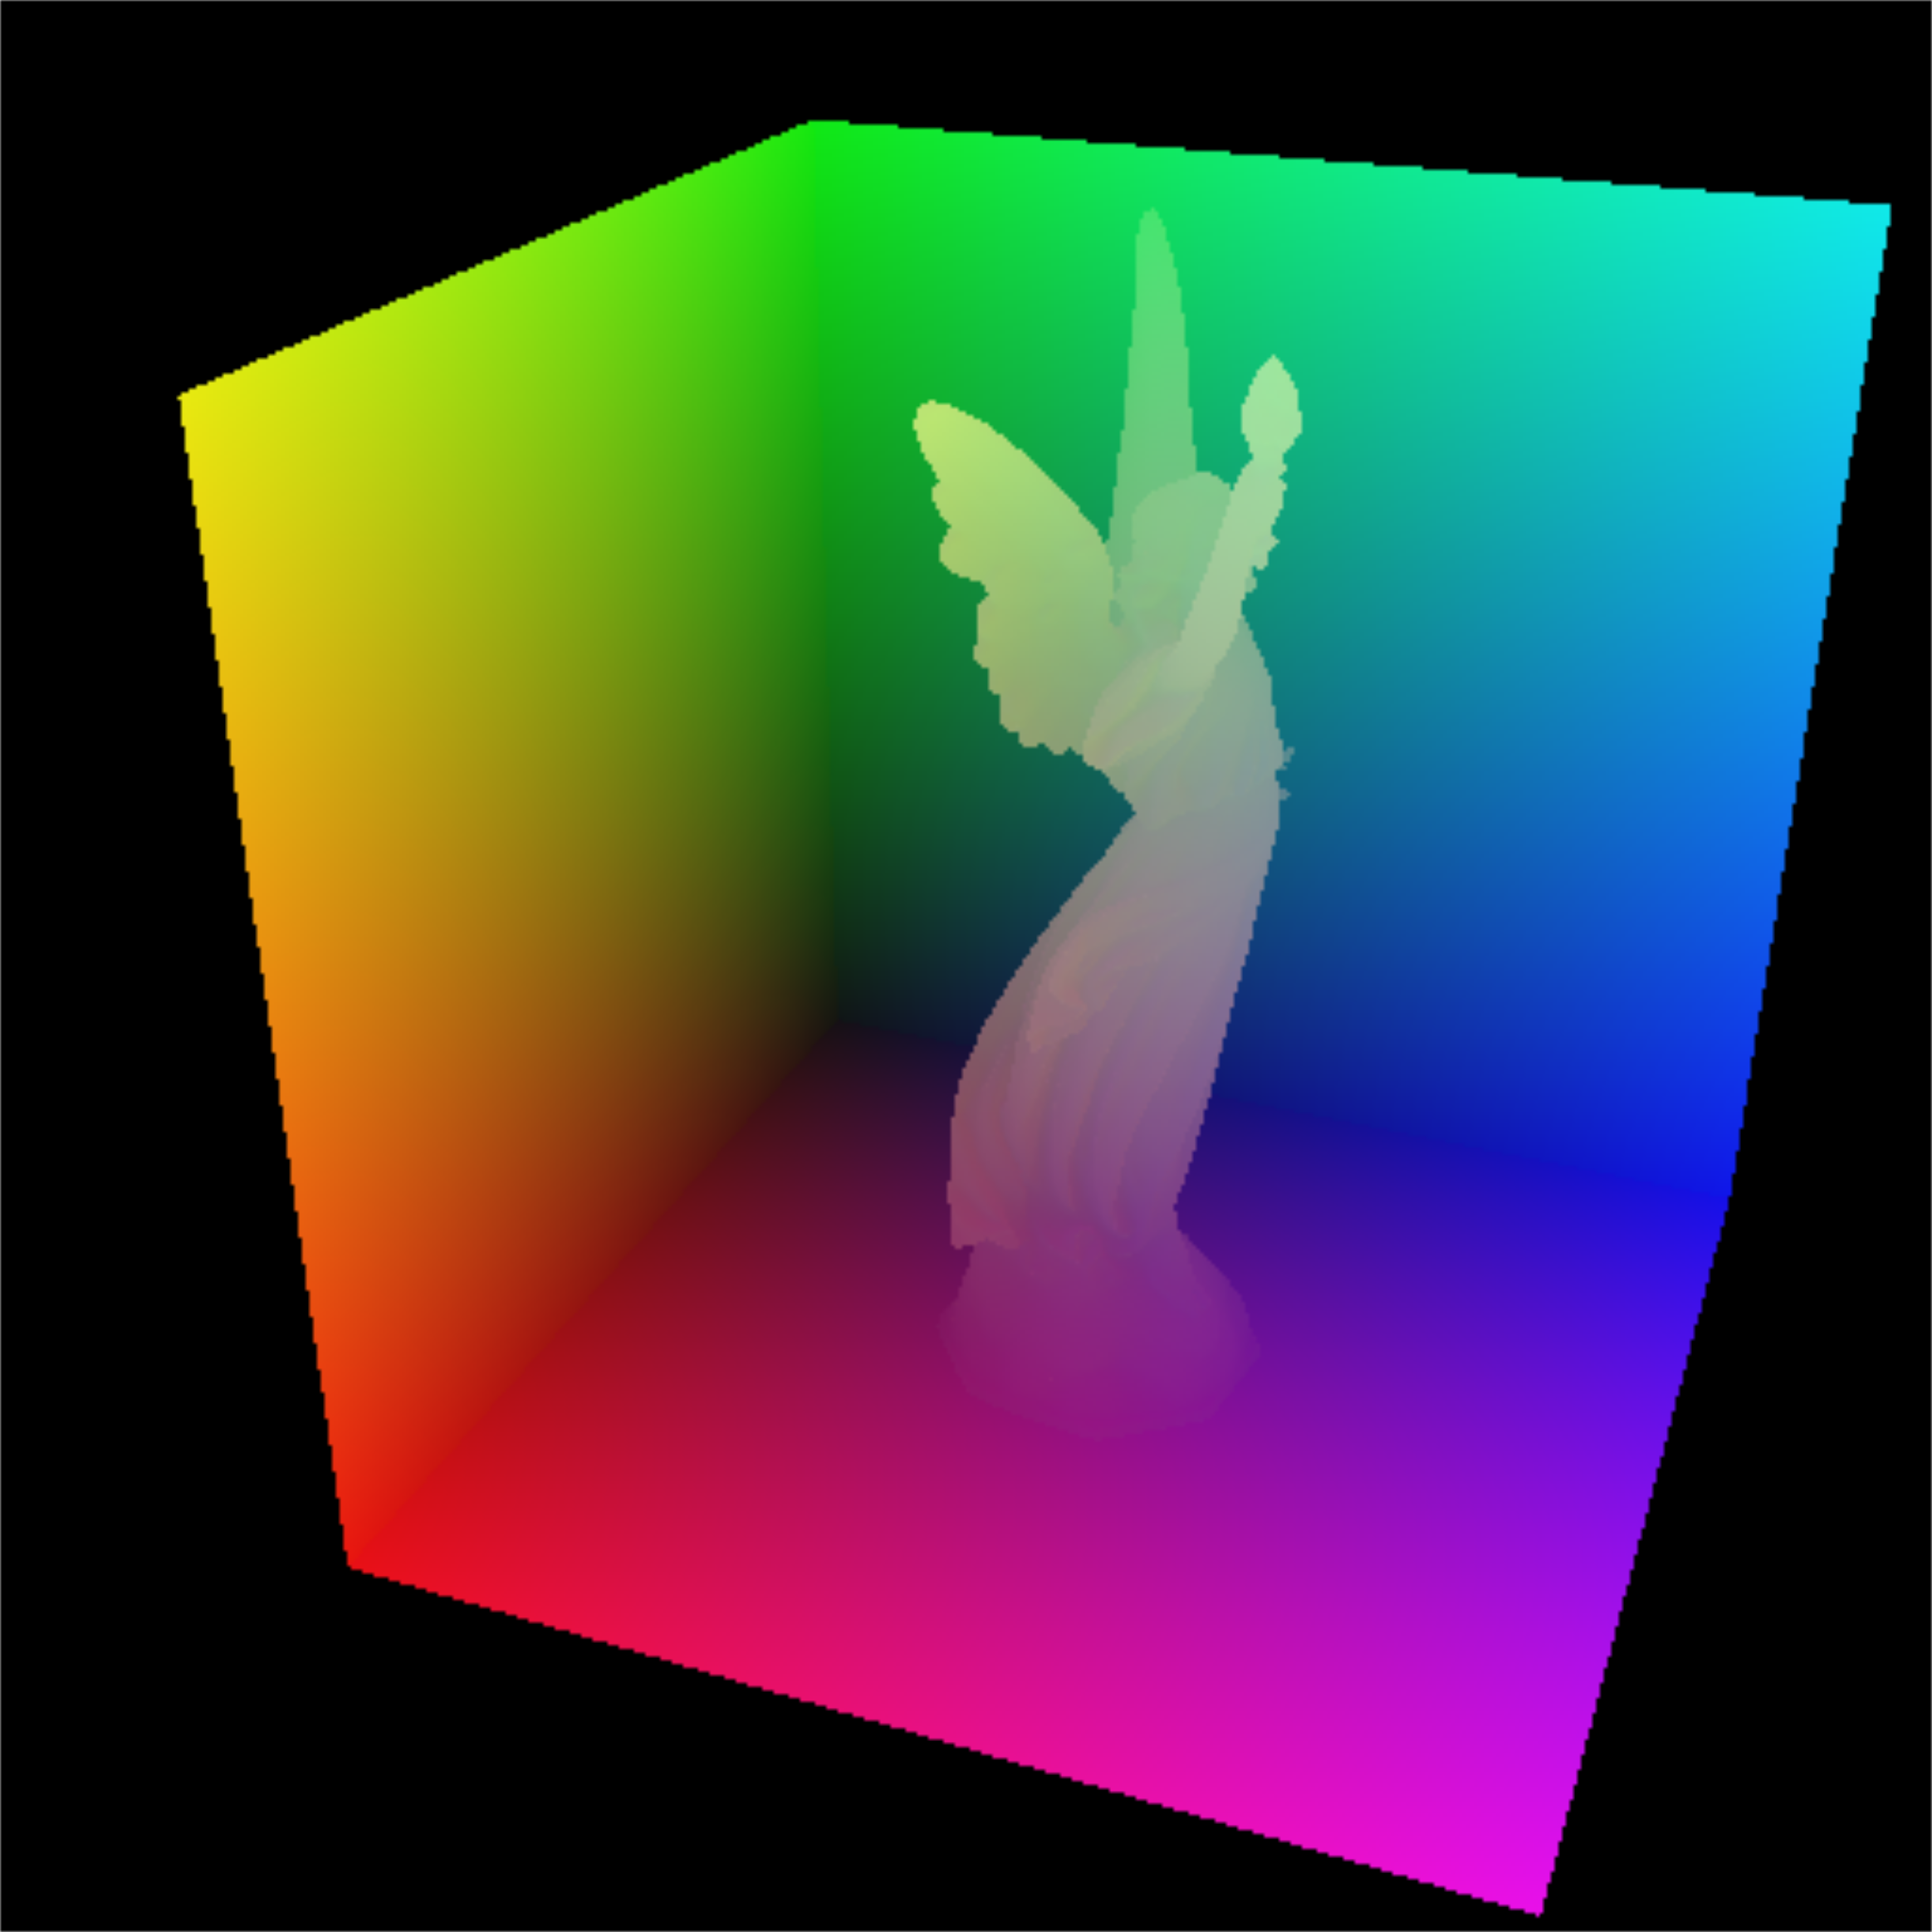
\includegraphics[width=\linewidth]{media/rsmp.png}
		\caption*{Posición.}
	\end{subfigure}
	\begin{subfigure}[t]{.24\linewidth}
		\centering
		\captionsetup{justification=centering}
		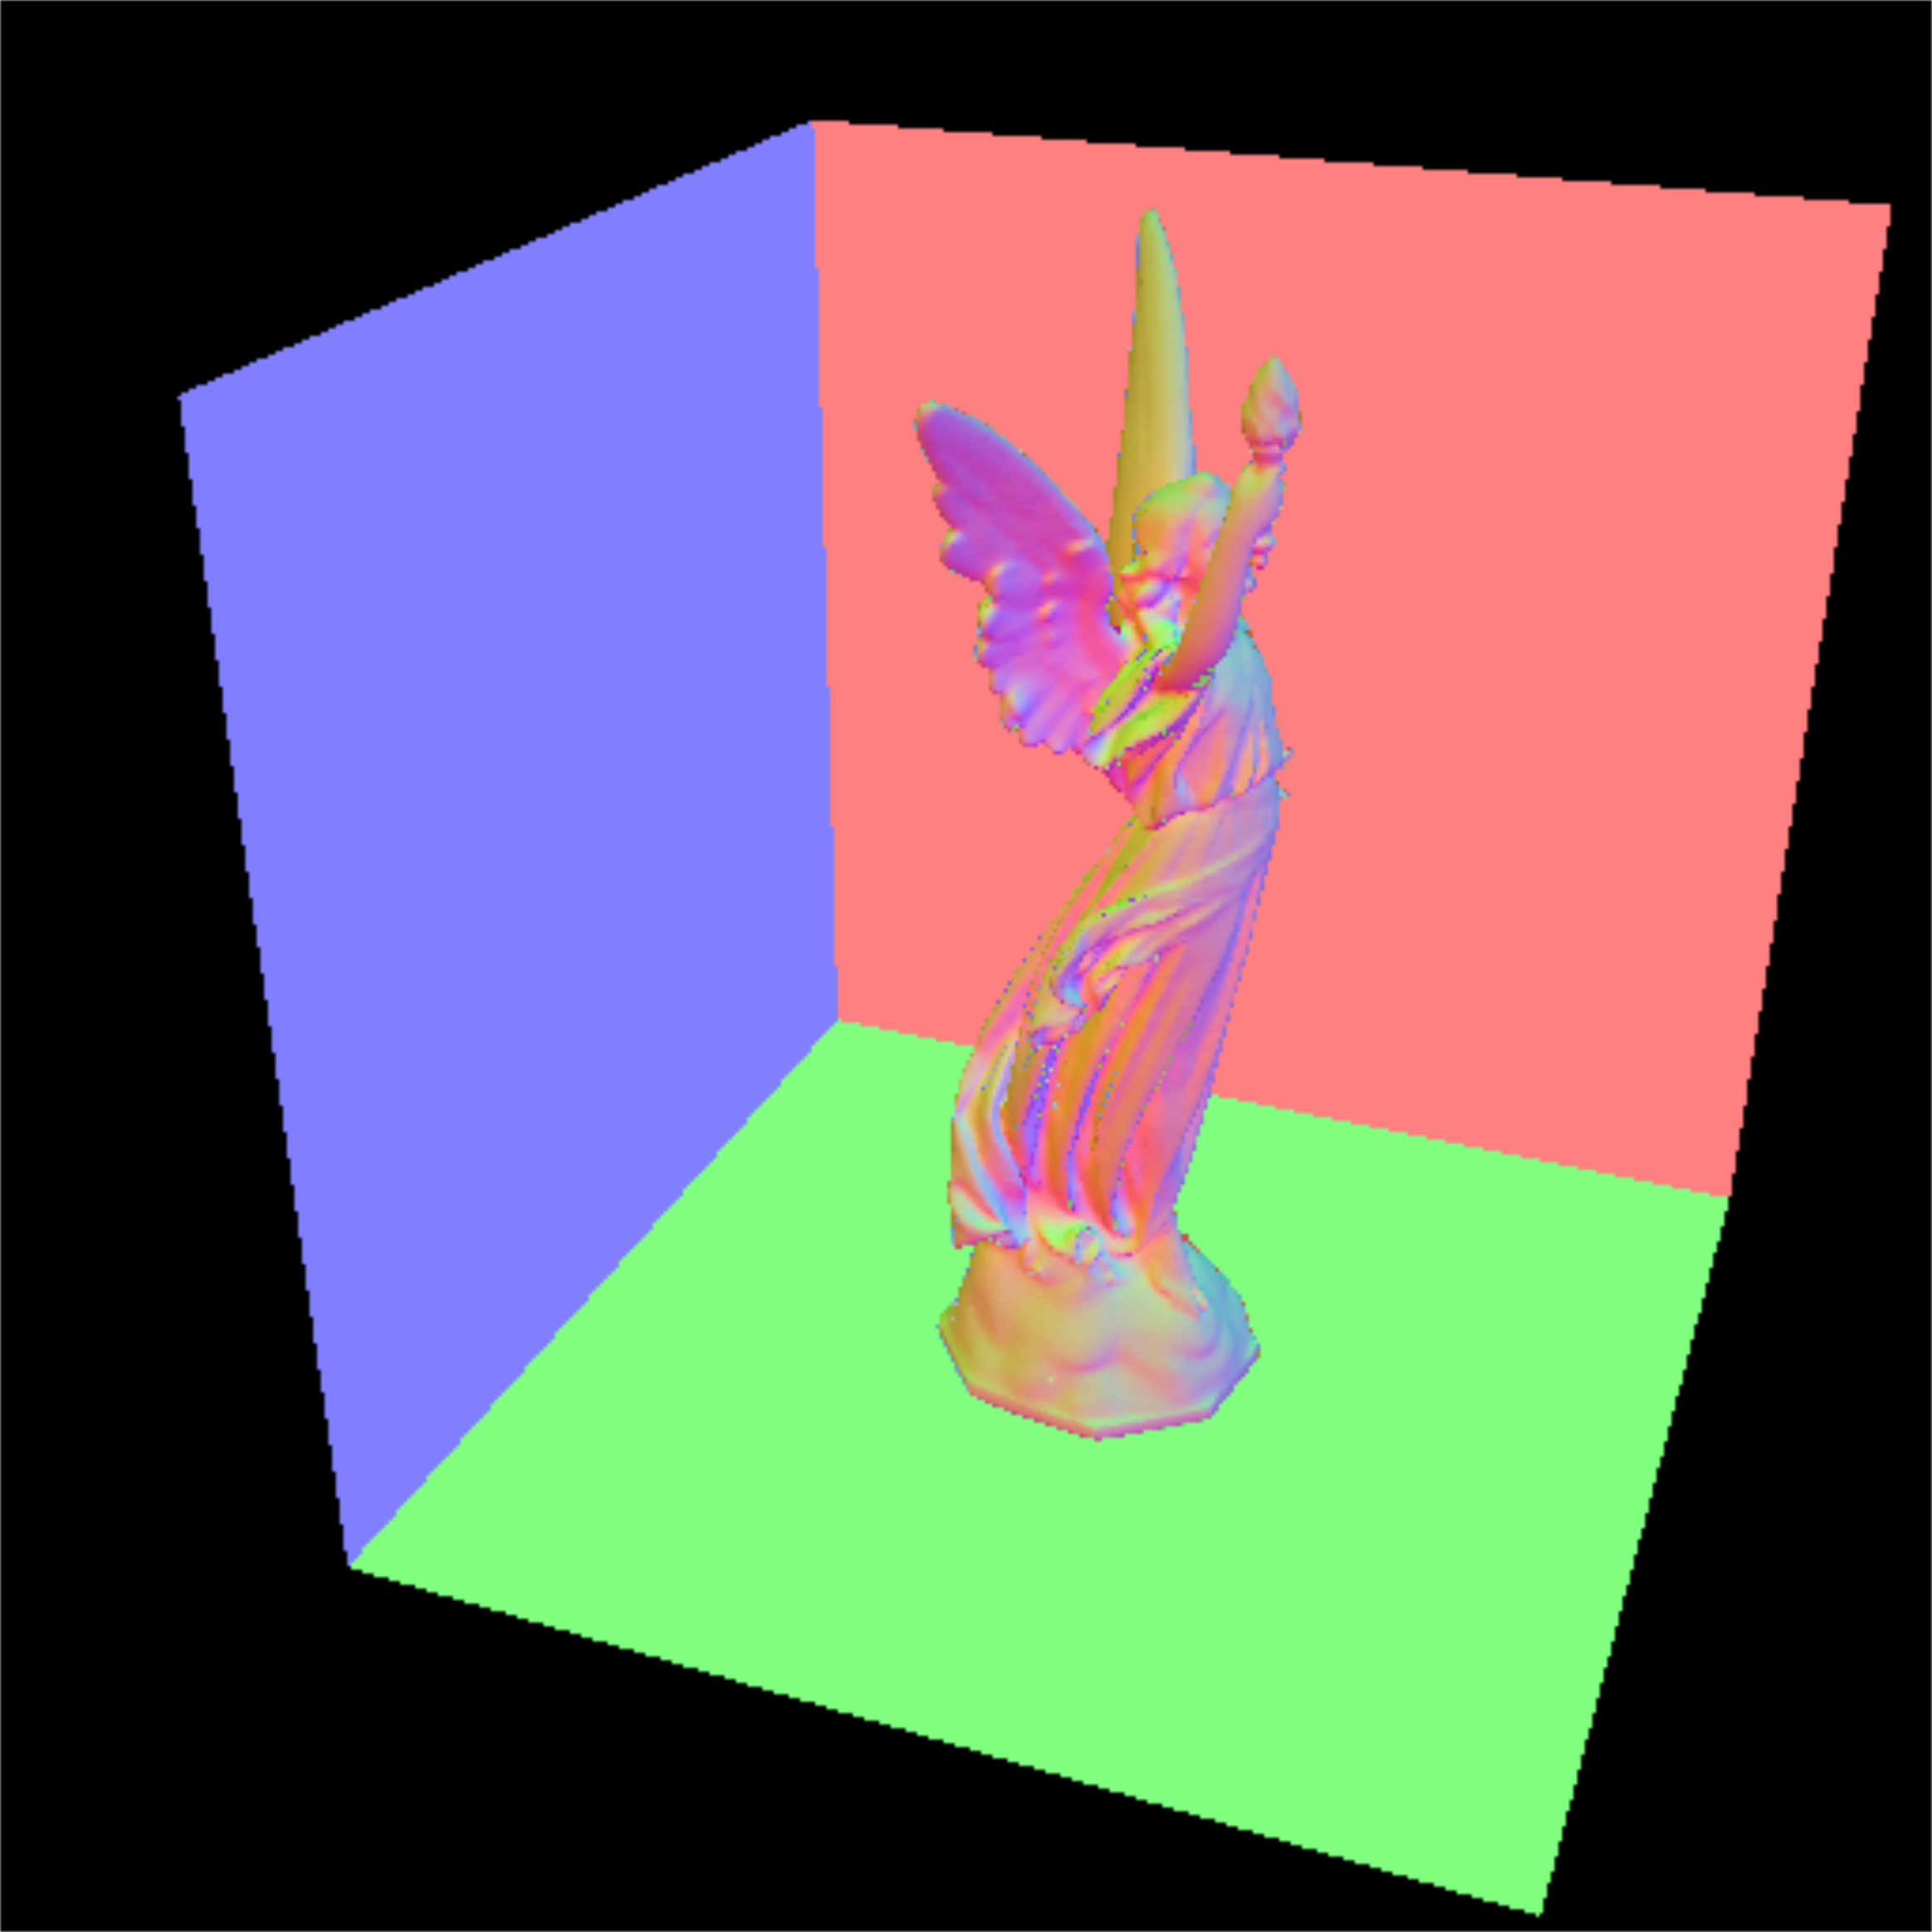
\includegraphics[width=\linewidth]{media/rsmn.png}
		\caption*{Normal.}
	\end{subfigure}
	\begin{subfigure}[t]{.24\linewidth}
		\centering
		\captionsetup{justification=centering}
		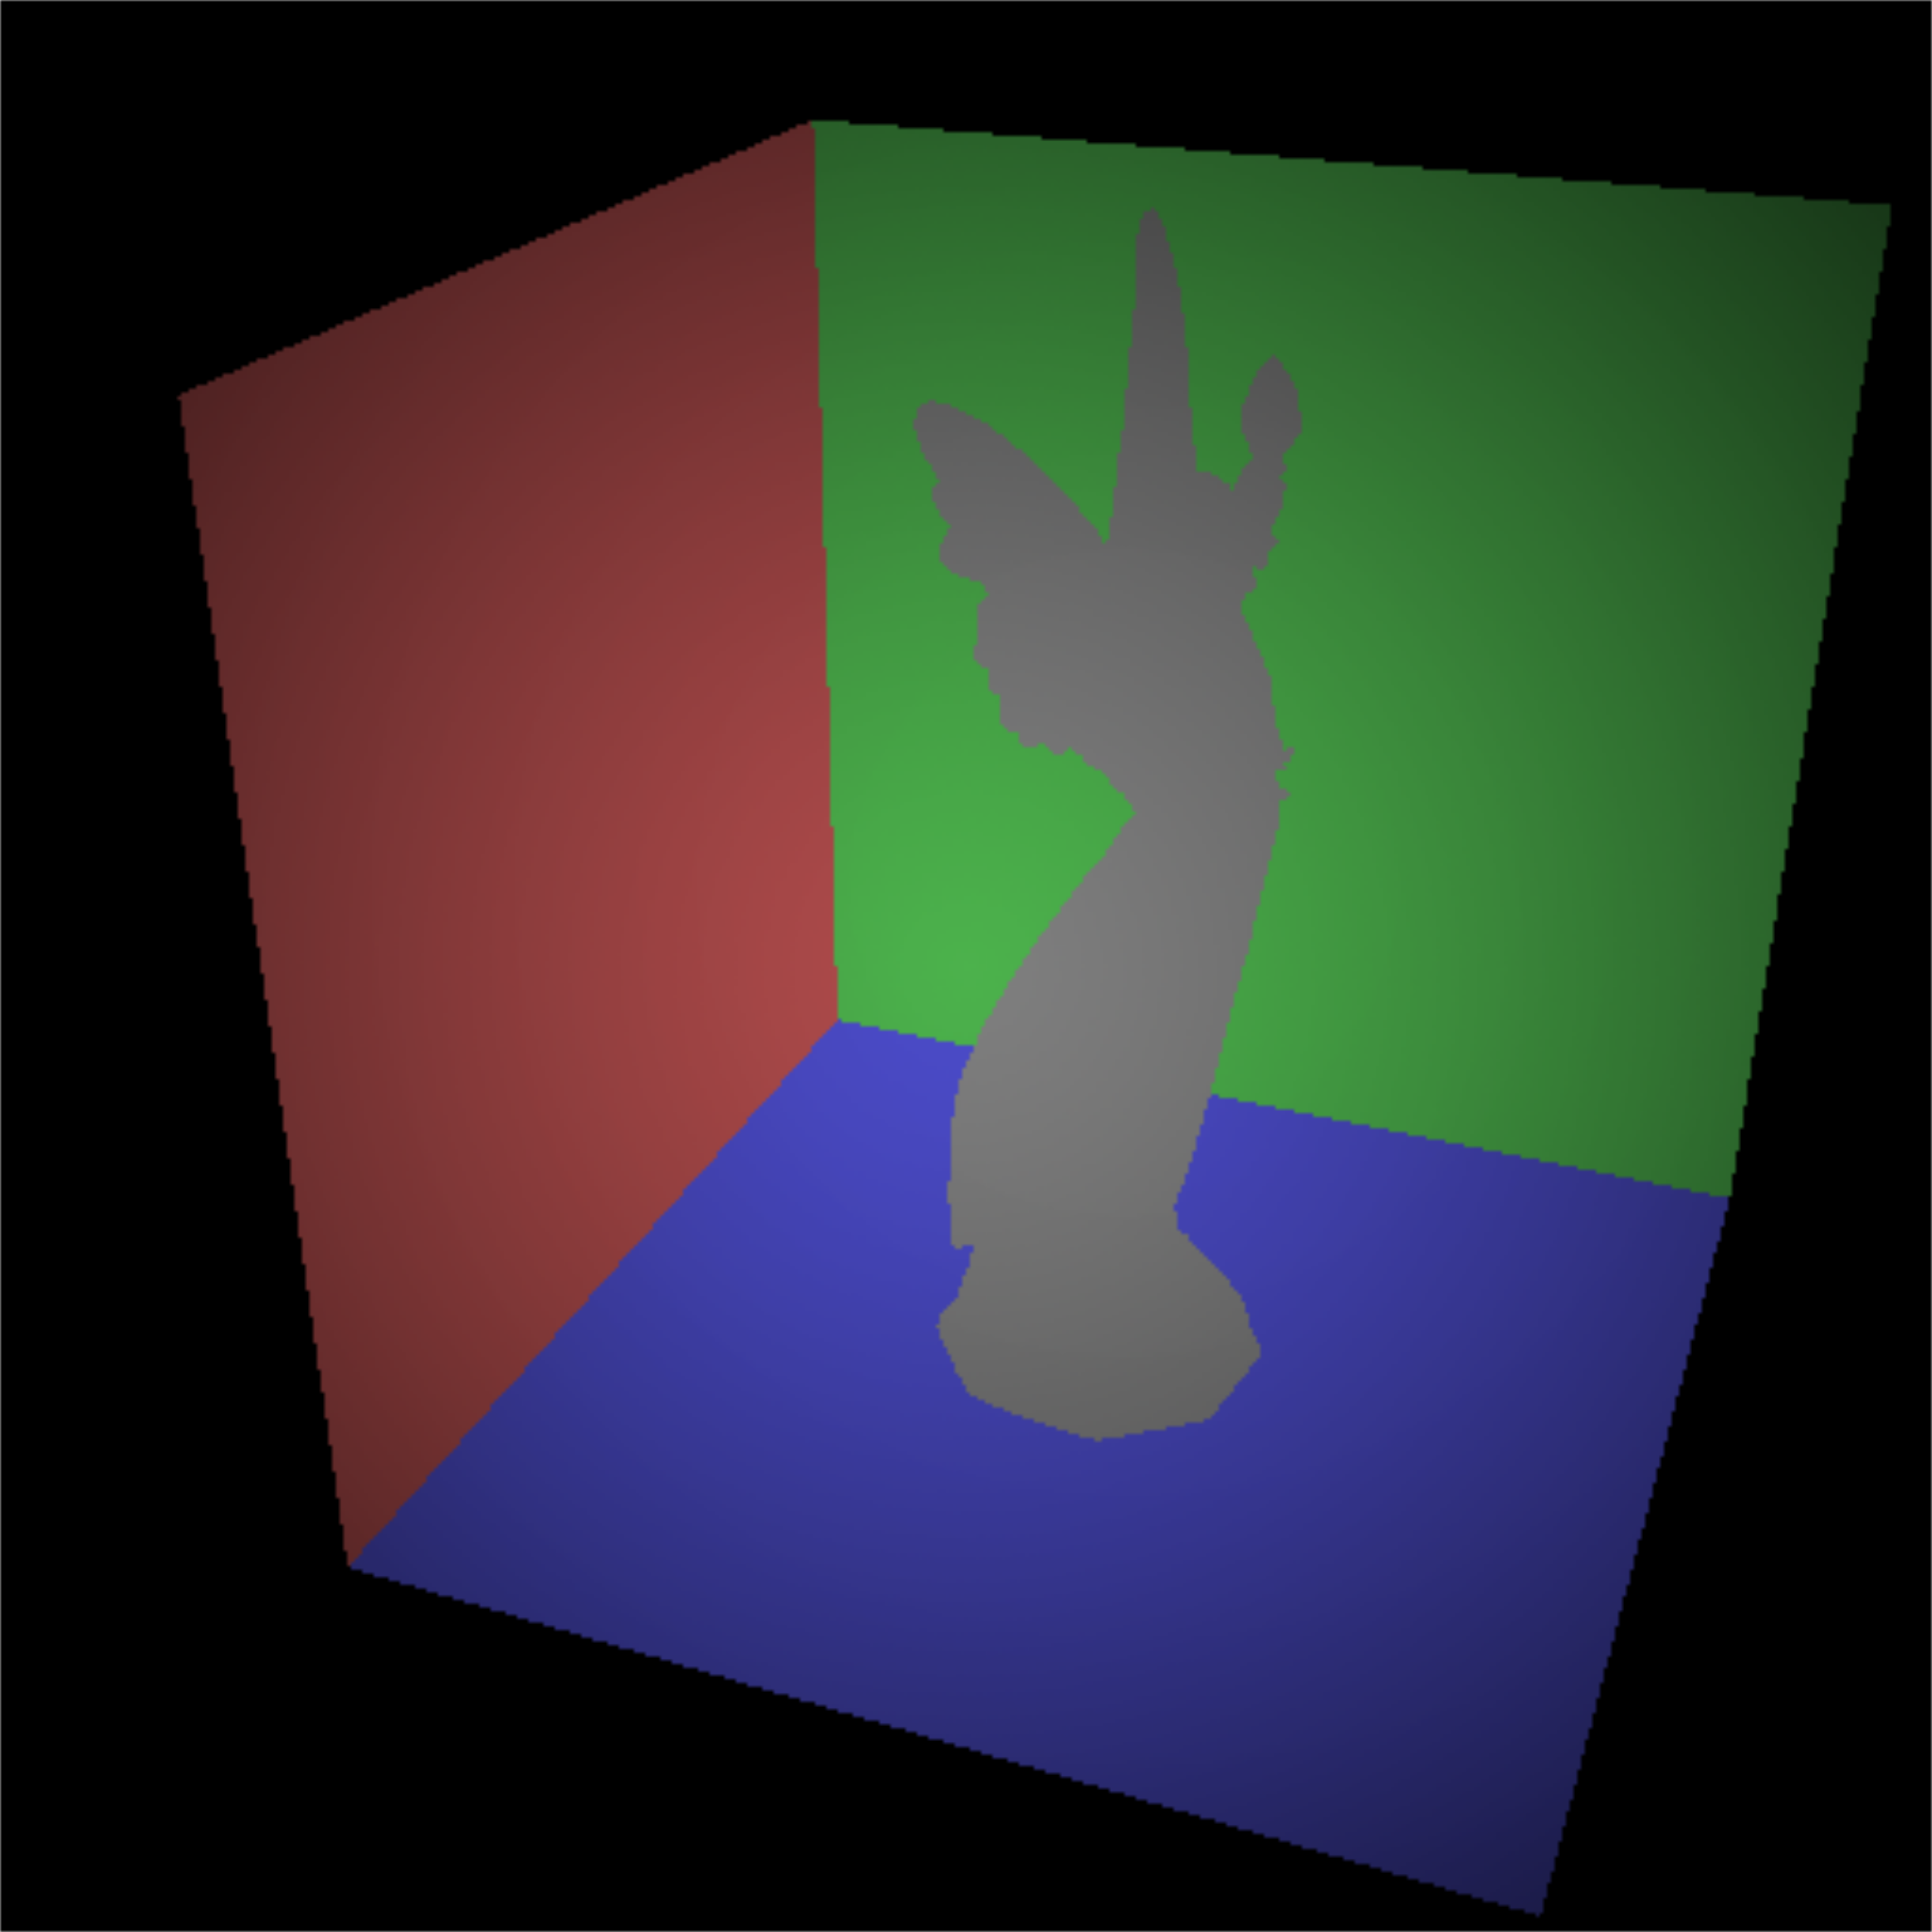
\includegraphics[width=\linewidth]{media/rsmf.png}
		\caption*{Flujo de radiancia.}
	\end{subfigure}
	\caption{Mapas utilizados por \ac{RSM} \cite{Dachsbacher:2005}.}
	\label{fig:rsm_fbo}
\end{figure}

Si se asume que todas las superficies son reflectores difusos, la intensidad de la radiancia emitida en una dirección $\omega$ desde un píxel del \ac{RSM} es descrita por la siguiente ecuación:

\begin{equation}
    I_{p}(\omega) = \Theta_{p}max(0, n_{p} \cdot {w})
    \label{eq:rsm_radiance}
\end{equation}

La iluminación indirecta de un punto se calcula sumando todas las intensidades de todos los píxeles (considerados ahora como luces) en el \ac{RSM} visibles. Calcular esto es costoso, por tanto en vez sumar todos los píxeles visibles al punto se toma cierta cantidad de muestras del \ac{RSM}. La posición del punto iluminado $x_{p}$ es proyectado sobre el \ac{RSM} y las muestras son seleccionadas alrededor de esta posición proyectada. La densidad de las muestras decrece con la distancia cuadrada de la posición proyectada al punto iluminado. Esto asume que dos superficies cercanas proyectadas al \ac{RSM} también son cercanas en el \ac{RSM}. También se asume que la muestra es directamente visible desde la superficie iluminada.

\subsection{Volúmenes de Propagación de Luz en Cascada}
\label{sub:clpv}
\Ac{CLPV} o \emph{Cascaded Light Propagation Volumes} presentando por Kaplanyan et al. en 2010 \cite{Kaplanyan:2010} es un algoritmo para el cálculo de iluminación indirecta difusa en tiempo real. En la Figura \ref{fig:lvp_results} se observan los resultados de esta técnica.

\begin{figure}[H]
	\centering
	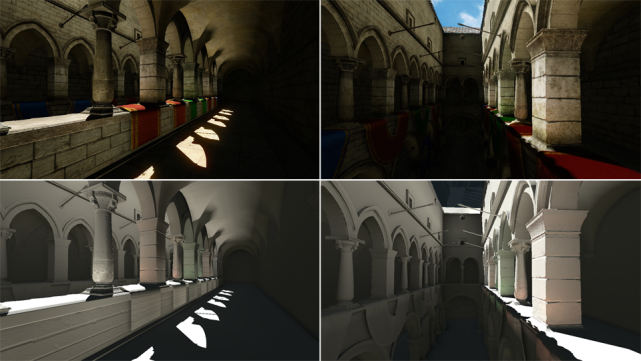
\includegraphics[width=0.85\linewidth]{media/lpvresult.png}
	\caption{Iluminación global para la escena \emph{Sponza} utilizando volúmenes de propagación de luz \cite{Kaplanyan:2010}.}
	\label{fig:lvp_results}
\end{figure}

\begin{wrapfigure}[11]{l}{0.3\linewidth}
	\centering
	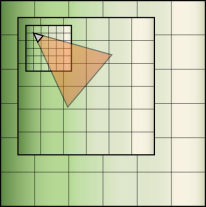
\includegraphics[width=0.90\linewidth]{media/g4957.png}
	\caption{Cuadrículas de \\ propagación anidadas, las cuadrículas se solapan.}
	\label{fig:nested_lpv}
\end{wrapfigure}
\noindent Este método simula el transporte de luz utilizando técnicas similares en algoritmos para simulación de fluidos basados en cuadrículas tridimensionales \cite{Crane07}. La intensidad de luz es almacenada en una cuadrícula y de forma iterativa cada celda transfiere la intensidad de la luz a sus vecinos. Esta cuadrícula es llamada \ac{LPV}. La luz puede ser bloqueada por la geometría de la escena, la cual es obtenida de otra cuadrícula llamada \ac{GV}. Para mejorar el rendimiento del algoritmo y reducir el consumo de memoria se utiliza un conjunto de cuadrículas anidadas (ver Figura \ref{fig:nested_lpv}). Para los objetos cercanos al observador la iluminación indirecta es calculada utilizando una cuadrícula mucho más fina.

Primero por cada fuente de luz, es necesario renderizar un \ac{RSM}. Cada texel del \ac{RSM} es considerado una \ac{VPL}. La intensidad del \ac{VPL} es acumulada y almacenada como un harmónico esférico dentro de las celdas de la cuadrícula.

Para una correcta propagación de la luz el algoritmo necesita conocer la geometría de la escena. Por esto de la misma manera en la que se almacena la intensidad de la luz también se almacena una representación de la escena en una cuadrícula. Esta representación es guardada sobre el \ac{GV}. Esta cuadrícula es trasladada por la mitad del tamaño de una celda con respecto al \ac{LPV}, esto asegura que el centro de todas las celdas del \ac{GV} queden en las esquinas del \ac{LPV}. Para conocer segmentos de geometría se utiliza un \ac{GBuffer} y las fuentes de luz de los \ac{RSM}s.


\begin{figure}[H]
	\centering
	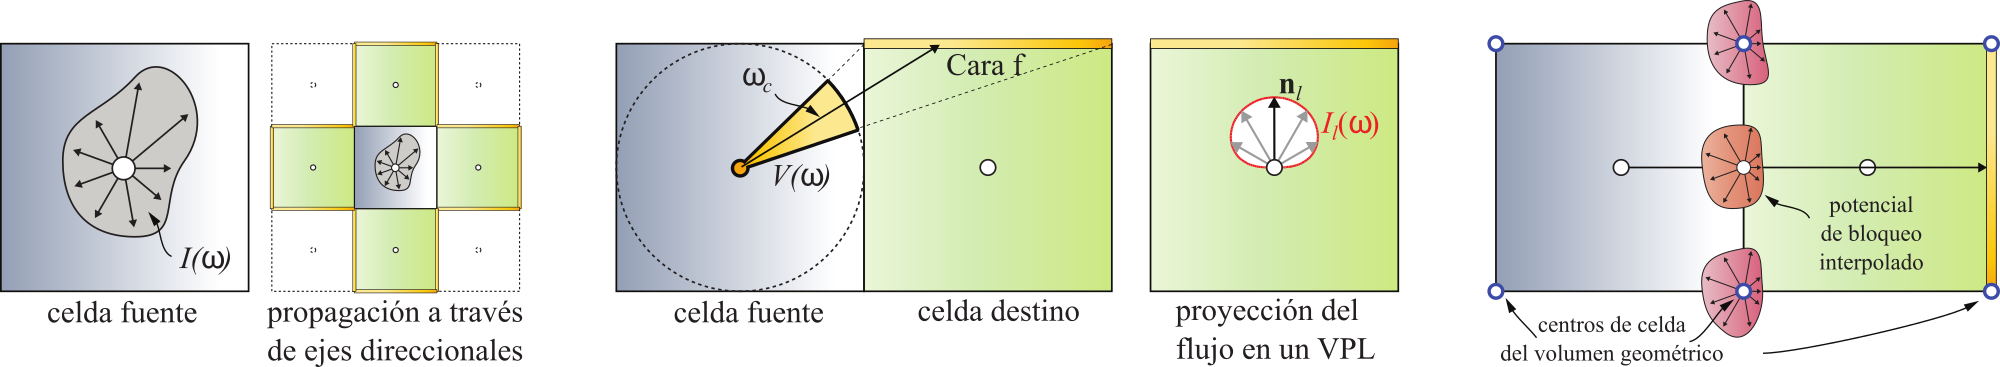
\includegraphics[width=\linewidth]{media/lpv_explain.png}
	\caption{Izquierda: Cada celda del \ac{LPV} almacena la intensidad de luz que es propagada desde la celda fuente. Centro: El flujo es calculado sobre cada cara de la celda destino para preservar información direccional. Derecha: Oclusión borrosa o \emph{fuzzy} almacenando una representación volumétrica de la escena \cite{Kaplanyan:2010}.}
	\label{fig:lpv_explain}
\end{figure}

La propagación de luz se realiza de forma iterativa. La intensidad de luz en cada iteración es propagada a 6 vecinos por celda según eje direccional principal. Primero por cada celda adyacente el flujo de radiancia incidente por cada una de las celdas es calculado. Luego el flujo incidente de cada celda es transformado en emitancia radiante. Esto se logra creando \ac{VPL}s, cada una de estas luces virtuales son colocadas sobre una de las caras de la celda y emiten un flujo radiancia similar el flujo de radiancia de la celda. Estas \ac{VPL} son acumuladas dentro del \ac{LPV} de nuevo y almacenadas como esféricos harmónicos utilizando el mismo proceso de inyección del primer paso. En la Figura \ref{fig:lpv_explain} se describe este algoritmo. 

\subsection{Iluminación Indirecta con Trazado de Conos y Vóxeles}
\label{sub:voxel_cone_tracing_orig}
Este algoritmo es presentado por Crassin et al. en 2011 \cite{CNSGE11b} para el cálculo de iluminación indirecta utilizando trazado de conos contra vóxeles o \emph{Indirect Illumination Using Voxel Cone Tracing}. En la Figura \ref{fig:givoxels_sponzanew1} se observan los resultados de este algoritmo. En esta técnica se utiliza una estructura de árbol disperso o \emph{sparse} para almacenar ya filtrados los valores necesarios para el cálculo de iluminación indirecta en vóxeles. Este árbol es una representación tridimensional de la escena por tanto cada nodo tiene ocho hijos que representan las ocho particiones de un cubo en partes más pequeñas de forma uniforme. Esta clase de estructuras son llamadas \emph{octrees}. La estructura dispersa requiere menor consumo de memoria ya que solo los vóxeles necesarios son almacenados.

\begin{figure}[H]
	\centering
	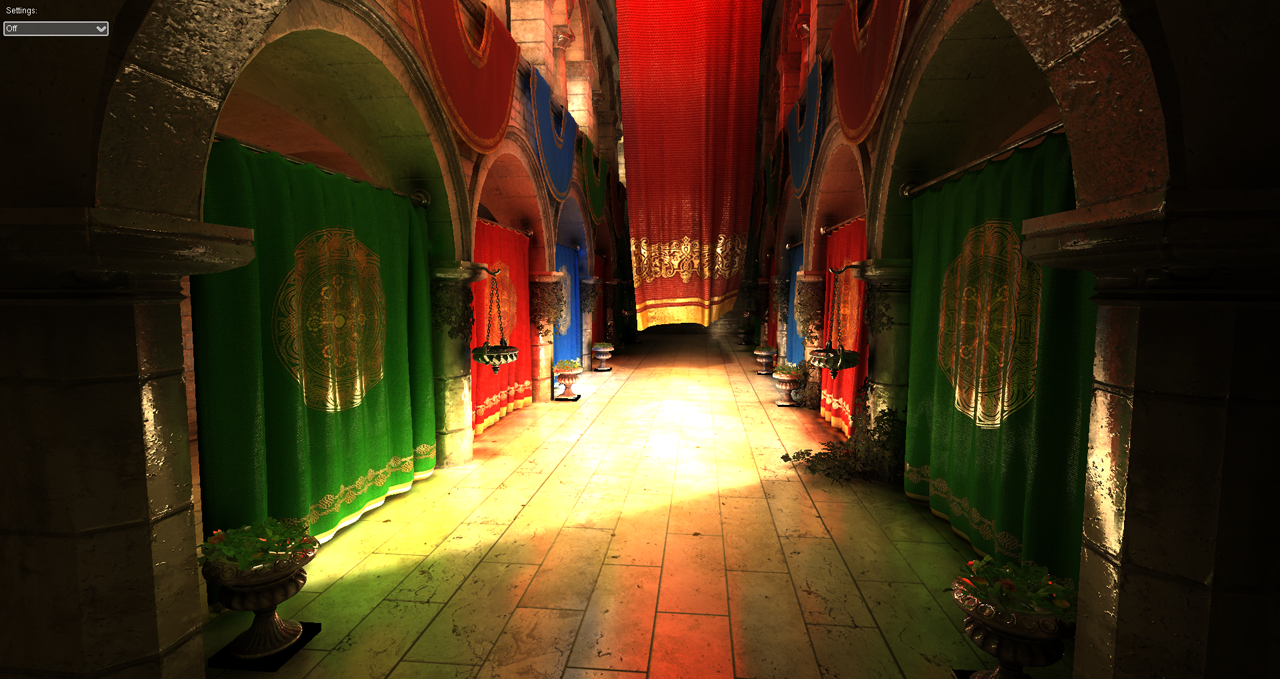
\includegraphics[width=0.9\linewidth]{media/givoxels_sponzanew1.png}
	\caption{Escena \emph{Sponza} renderizada utilizando trazado de conos con vóxeles para la iluminación indirecta \cite{CNSGE11b}.}
	\label{fig:givoxels_sponzanew1}
\end{figure}

El algoritmo comprende varios pasos: primero la información de la luz y escena son almacenados en las hojas de la estructura de árbol, este es el nivel más fino de la jerarquía. Luego estos valores son filtrados dentro del árbol disperso hacia todos los niveles de la jerarquía hasta llegar a la raíz. En un último paso para el cálculo de iluminación indirecta por cada fragmento, los valores dentro de esta jerarquía son recolectados sobre una semiesfera utilizando trazado de conos. En algoritmos como ray tracing esta recolección de valores es lenta y es realizada por muchos rayos. Es de notar que todos estos rayos trazados sobre la semiesfera son direccional y espacialmente coherentes. \Ac{VCT} hace uso de este concepto para discretizar muchos rayos en simples conos.

\subsubsection{Construcción del Octree de Vóxeles}
\label{subsub:octree_building}
El algoritmo está pensando para funcionar con escenas dinámicas. Sin embargo las escenas son divididas entre partes dinámicas y estáticas para acelerar el proceso de voxelización con objetos dinámicos.

Primero la escena es renderizada utilizando proyección ortogonal. Cada triángulo es proyectado sobre uno de los ejes principales, este eje es seleccionado según la normal del triángulo, esto se hace para maximizar el área visible del triángulo con respecto al eje. Cada fragmento producto de esta proyección es almacenado en una lista de vóxeles-fragmentos junto a parámetros como posición en escena, normal y color. Para saber la cantidad de elementos que esta lista debe almacenar primero se debe realizar una pasada contando el número de fragmentos con un contador atómico.

\begin{wrapfigure}{l}{0.4\linewidth}
	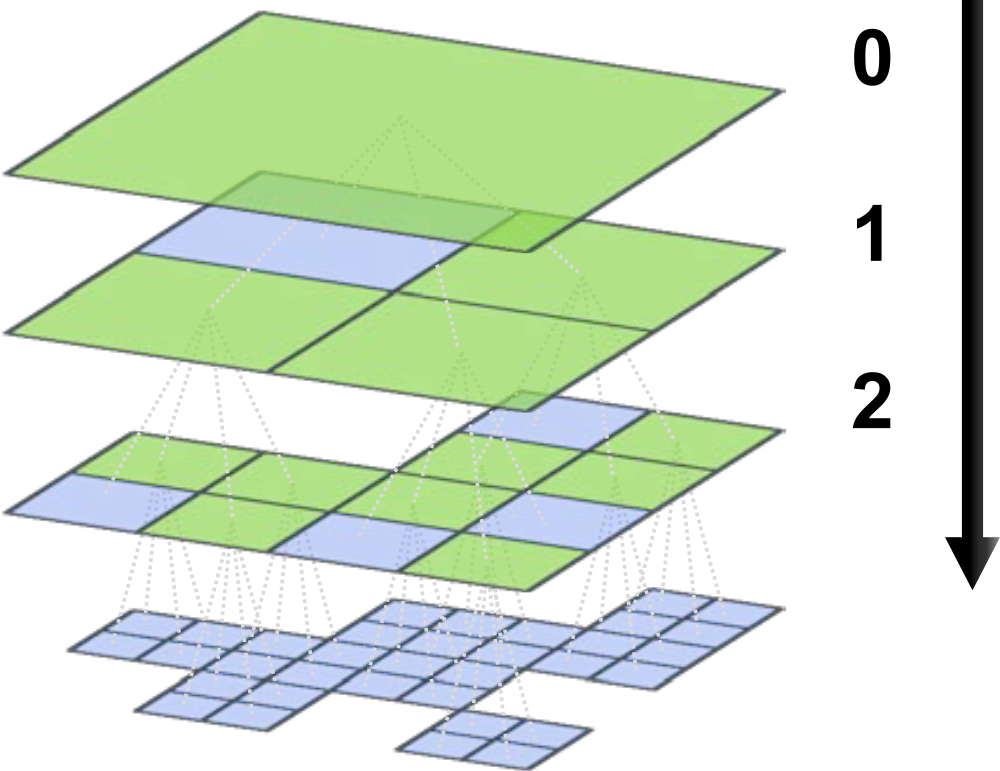
\includegraphics[width=0.95\linewidth]{media/miplevels.png}
	\caption{Descripción gráfica del proceso de subdivisión del octree.}
	\label{fig:miplevels}
\end{wrapfigure}
\noindent Una vez llena la lista de vóxeles-fragmentos, se genera un hilo de procesamiento por cada fragmento en la lista. Los fragmentos son introducidos en el árbol disperso que inicialmente solo tiene un nodo raíz (ver Figura \ref{fig:miplevels}). Cada vez que un nodo de este octree necesita ser dividido un nuevo nodo es creado y se almacena sobre memoria ya reservada en la \ac{GPU}. La posición del nodo en memoria es determinada por un contador atómico, el cual se incrementa con cada nuevo nodo. Al inicio del proceso de subdivisión de los nodos se genera una gran cantidad de colisiones entre hilos, por esto cada nodo tiene asociado un símbolo mutex.

\subsubsection{Contenido de un Vóxel}
\label{subsub:voxelcontent_orig}

El algoritmo está diseñado para hacer uso de filtrado trilineal por hardware. Sin embargo dos vóxeles vecinos no necesariamente están posicionados de forma subsecuente en memoria. Por esto cada nodo contiene un bloque o \emph{brick}. Este bloque representa el entramado $3^3$ de la celda, donde estas celdas se encuentran en las esquinas de los hijos del nodo (ver Figura \ref{fig:bricks_vct}).

Cada vóxel representa varios parámetros, entre ellos color, opacidad, normal, intensidad, etc.

\begin{figure}[H]
	\centering
	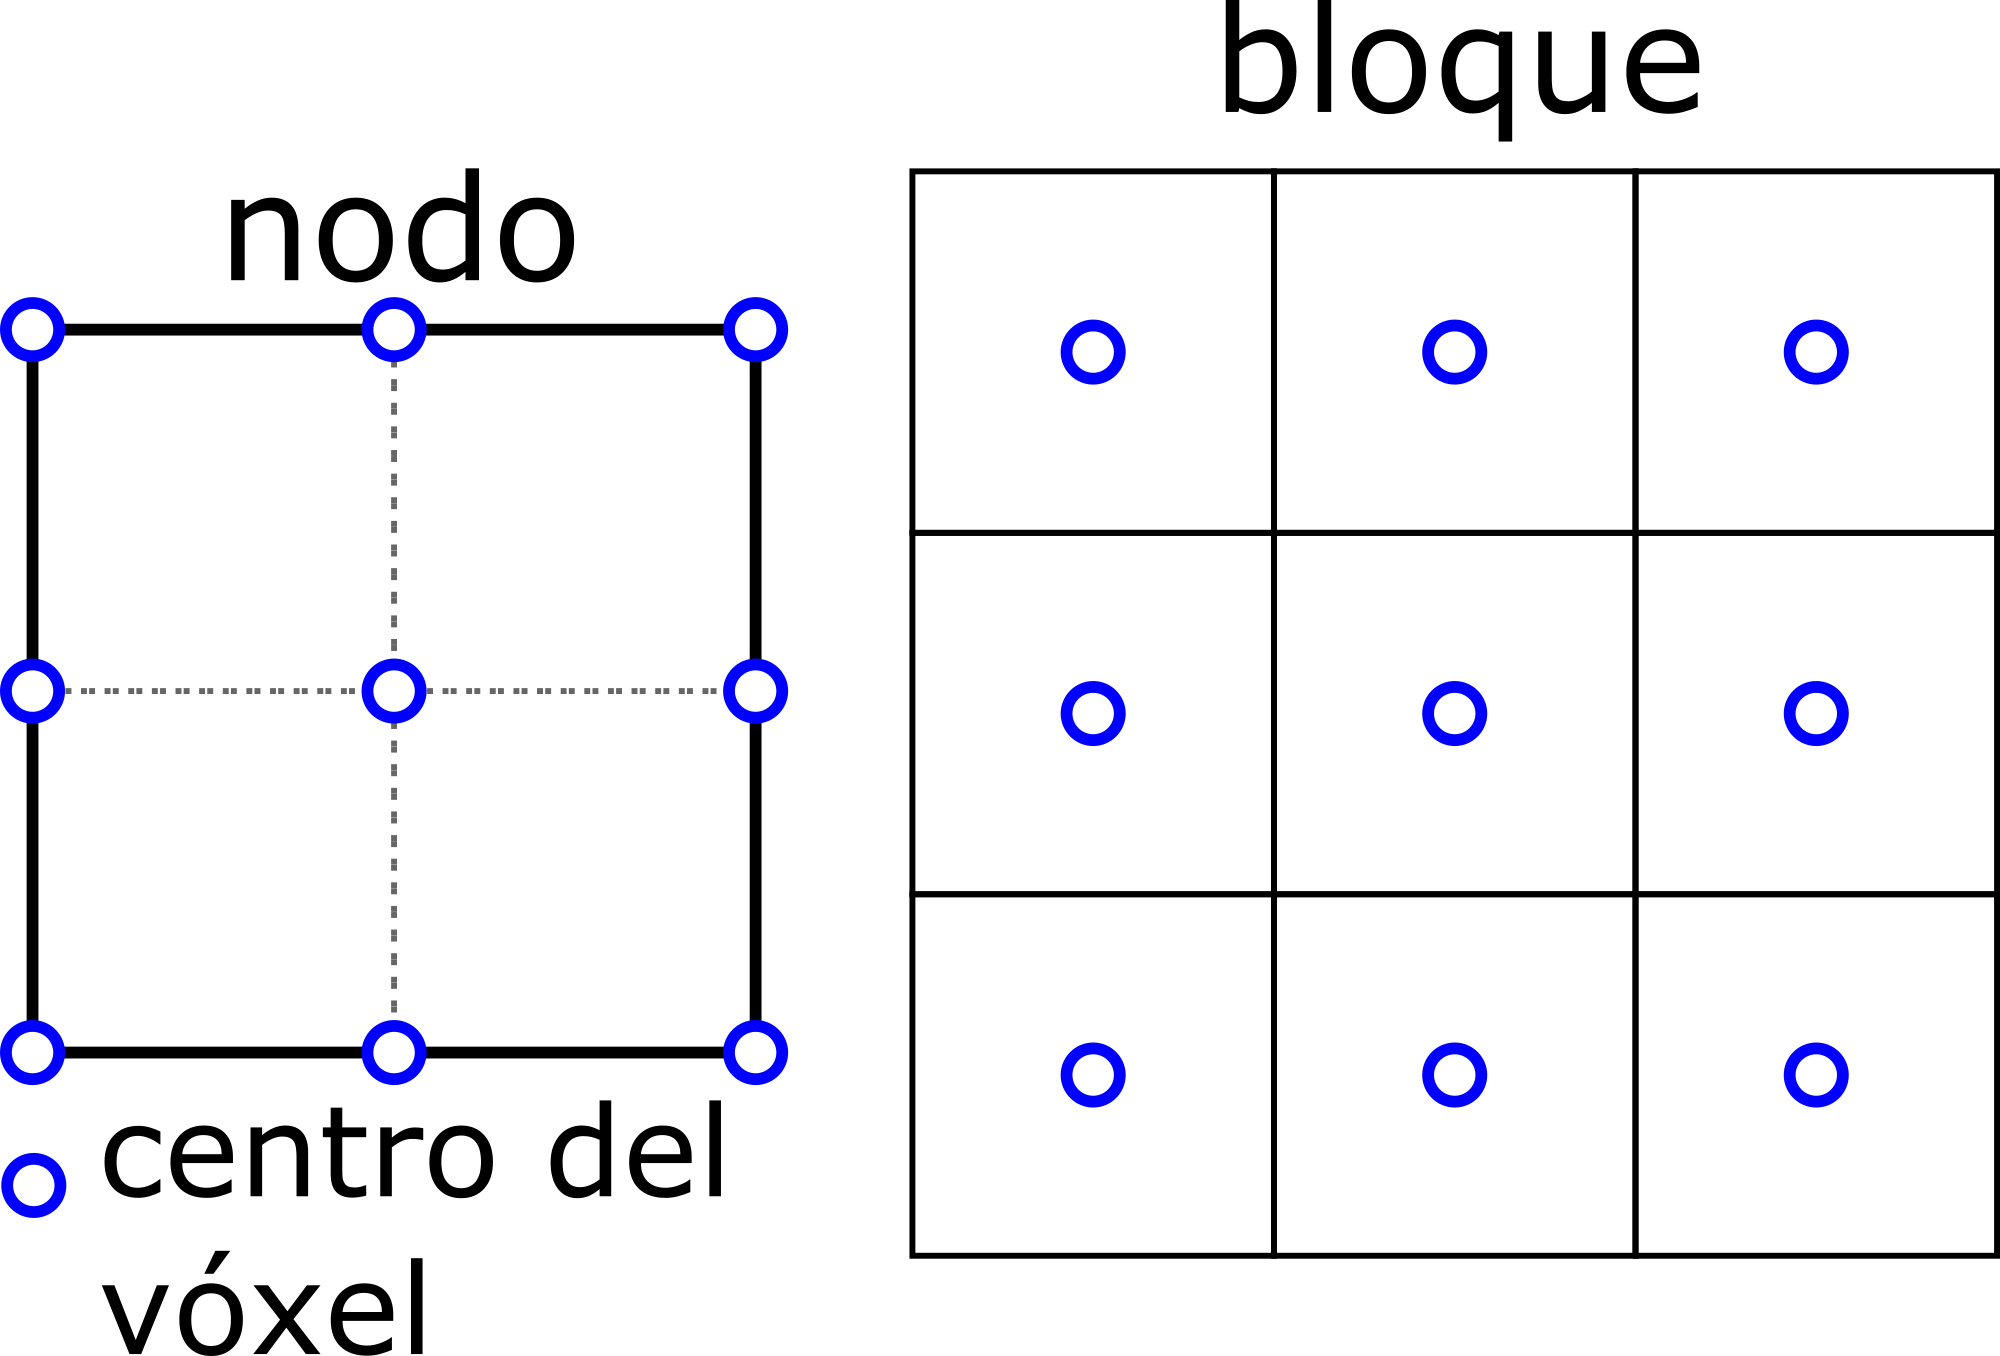
\includegraphics[width=0.3\linewidth]{media/bricks_vct.png}
	\caption{Bloques y nodos, los valores de los bloques se encuentran en las esquinas para rápido acceso y filtrado \cite{CNSGE11b}.}
	\label{fig:bricks_vct}
\end{figure}

\subsubsection{Filtrado Mip-mapping}
\label{subsub:mipmaping_orig}
Inicialmente cada uno de estos parámetros es almacenado dentro de las hojas del árbol disperso. Luego de forma iterativa estos valores son filtrados desde los niveles más bajos a los niveles más altos de la jerarquía, este proceso es llamado \emph{mip-mapping}. Cada nodo de un bloque es filtrado a partir de las $3^3$ celdas del nivel anterior en jerarquía. Para calcular el valor filtrado sobre el actual nodo el algoritmo promedia los valores de los nodos en el nivel anterior. Al calcular el valor filtrado cada vóxel debe ser pesado con la inversa de su multiplicidad, resultando en un kernel gaussiano de tamaño $3^3$. 

\subsubsection{Trazado de Conos y Vóxeles}
Una vez que el árbol disperso está filtrado y completo se utiliza para el cálculo de iluminación indirecta. Por cada fragmento un conjunto de conos es generado. La dirección y apertura de cada cono es determinada por la \ac{BRDF} del material en ese fragmento. Por ejemplo la \ac{BRDF} Blinn-Phong vista en la sección \ref{para:blinn_phong} puede ser descompuesta como un lóbulo ancho para la parte difusa y un lóbulo especular. Para el lóbulo difuso varios conos son generados orientados por la semiesfera sobre el punto con apertura y dirección maximizadas a tal manera que los conos cubran gran parte de la misma. Para el lóbulo especular se genera un solo cono con una apertura que varía según el término $n$ de la \ac{BRDF} Blinn-Phong. El cono especular tiene como dirección la dirección de la luz incidente reflectada $R$ (sección \ref{para:speculars}).

El algoritmo utiliza trazado de conos aproximados para acumular la intensidad de la luz incidente sobre el fragmento. Los valores son recolectados de varias muestras a través del recorrido del cono utilizando composicion \emph{front-to-back}. Por cada muestra se examina el árbol disperso de vóxeles. El nivel del árbol a examinar es determinado por el diámetro del cono en esa posición.

%Por cada paso del trazado se obtiene un valor de oclusión $\alpha_{2}$ y valor de radiancia $c_2$. Para acumular los valores en muestreados a través del recorrido del cono se utiliza acumulación volumétrica \emph{front-to-back}. Para esto es necesario llevar pista de un valor oclusión $a$ y color $c$. La actualización de estos valores por cada paso se realiza de la siguiente manera: $c=c+(1-a)c_2$ y $a=a+(1-a)a_2$

\subsubsection{Filtrado Anisotrópico de Vóxeles.}
\label{subsub:aniso_voxels_orig}
A pesar de que el filtrado gaussiano es suficiente para proveer resultados visuales coherentes, algunos problemas de calidad visual pueden ocurrir bajo ciertas condiciones. El primer problema se conoce como el problema de la pared rojo-verde. Al promediar valores dentro del octree con dos vóxeles opacos con diferentes colores provenientes de por ejemplo, dos paredes planas, el color resultante del vóxel describe ambas paredes como si estas fueran transparentes. Otro problema resulta también de promediar opacidad entre vóxeles totalmente transparentes y vóxeles totalmente opacos, resultando un valor filtrado semitransparente. Esto puede resultar en fugas de luz a través de la geometría en la escena.

\begin{figure}[H]
	\centering
	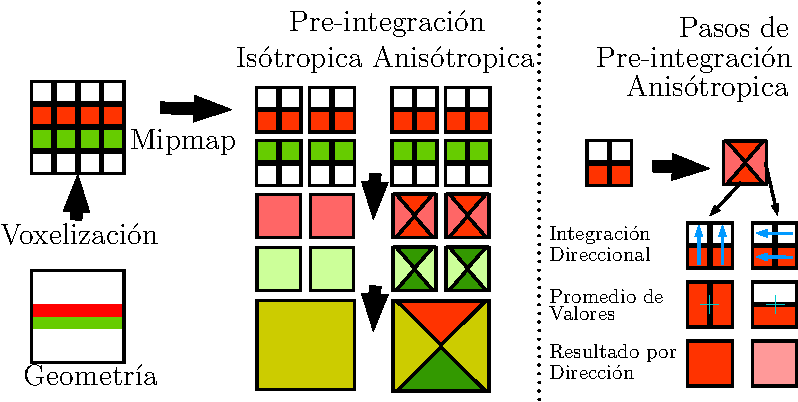
\includegraphics[width=0.90\linewidth]{media/isotropic_cropped.pdf}
	\caption{A la izquierda se describe el proceso de mipmapping de vóxeles sin y con filtrado anisótropico. Los pasos para la integración direccional se observan a la derecha.}
	\label{fig:vct_anisofiltering}
\end{figure}

Para solventar este problema se realiza una representación anisotrópica de los vóxeles durante el proceso de mip-mapping. En vez de tener un solo canal de valores filtrados sin dirección, ahora los valores serán filtrados de forma direccional, almacenando seis canales por cada eje positivo y negativo. Un valor direccional es calculado realizando un paso de integración volumétrica en profundidad y promediando los cuatro valores direccionales para obtener el valor resultante según una dirección (ver Fgura \ref{fig:vct_anisofiltering}).

\subsubsection{Captura de Iluminación Directa}
\label{subsub:voxel_capture}
Para el cálculo de iluminación indirecta es necesario describir como la radiancia incidente es almacenada en los nodos del árbol. Este proceso está inspirado en \ac{RSM}, donde la escena es renderizada desde el punto de vista de la fuente de luz y se utiliza rasterización estándar para almacenar las posiciones de los fragmentos en una textura. Cada píxel en esta textura representa un fotón que rebota en escena. Esta textura se le llama mapa de luz-vista o \emph{light-view map}. Luego de generar este mapa es necesario almacenar los fotones en el árbol octree. Los fotones son almacenados como una distribución direccional y energía proporcional al casquete esférico del ángulo solido del píxel visto desde la luz.

El procesamiento de la textura de fotones sobre el árbol se realiza en el procesador de fragmentos o \emph{fragment shader}. Como usualmente la dimensión del \emph{light-view map} es mayor a la resolución de la cuadrícula de vóxeles se puede asumir que los fotones serán almacenados directamente en las hojas del árbol octree. Además, los fotones siempre pueden ser almacenados en el nivel más fino de detalle en la representación con vóxeles porque estos describen información de la superficie geométrica. Es posible que muchos fotones terminen sobre un mismo vóxel, por esto es necesario utilizar adicción atómica para garantizar coherencia entre los hilos generados por cada fragmento.
